\section{Results and discussion}\label{sec:discussion}

\begin{figure*}[t!]
  \centering
\begin{subfigure}[t]{0.29\textwidth}
  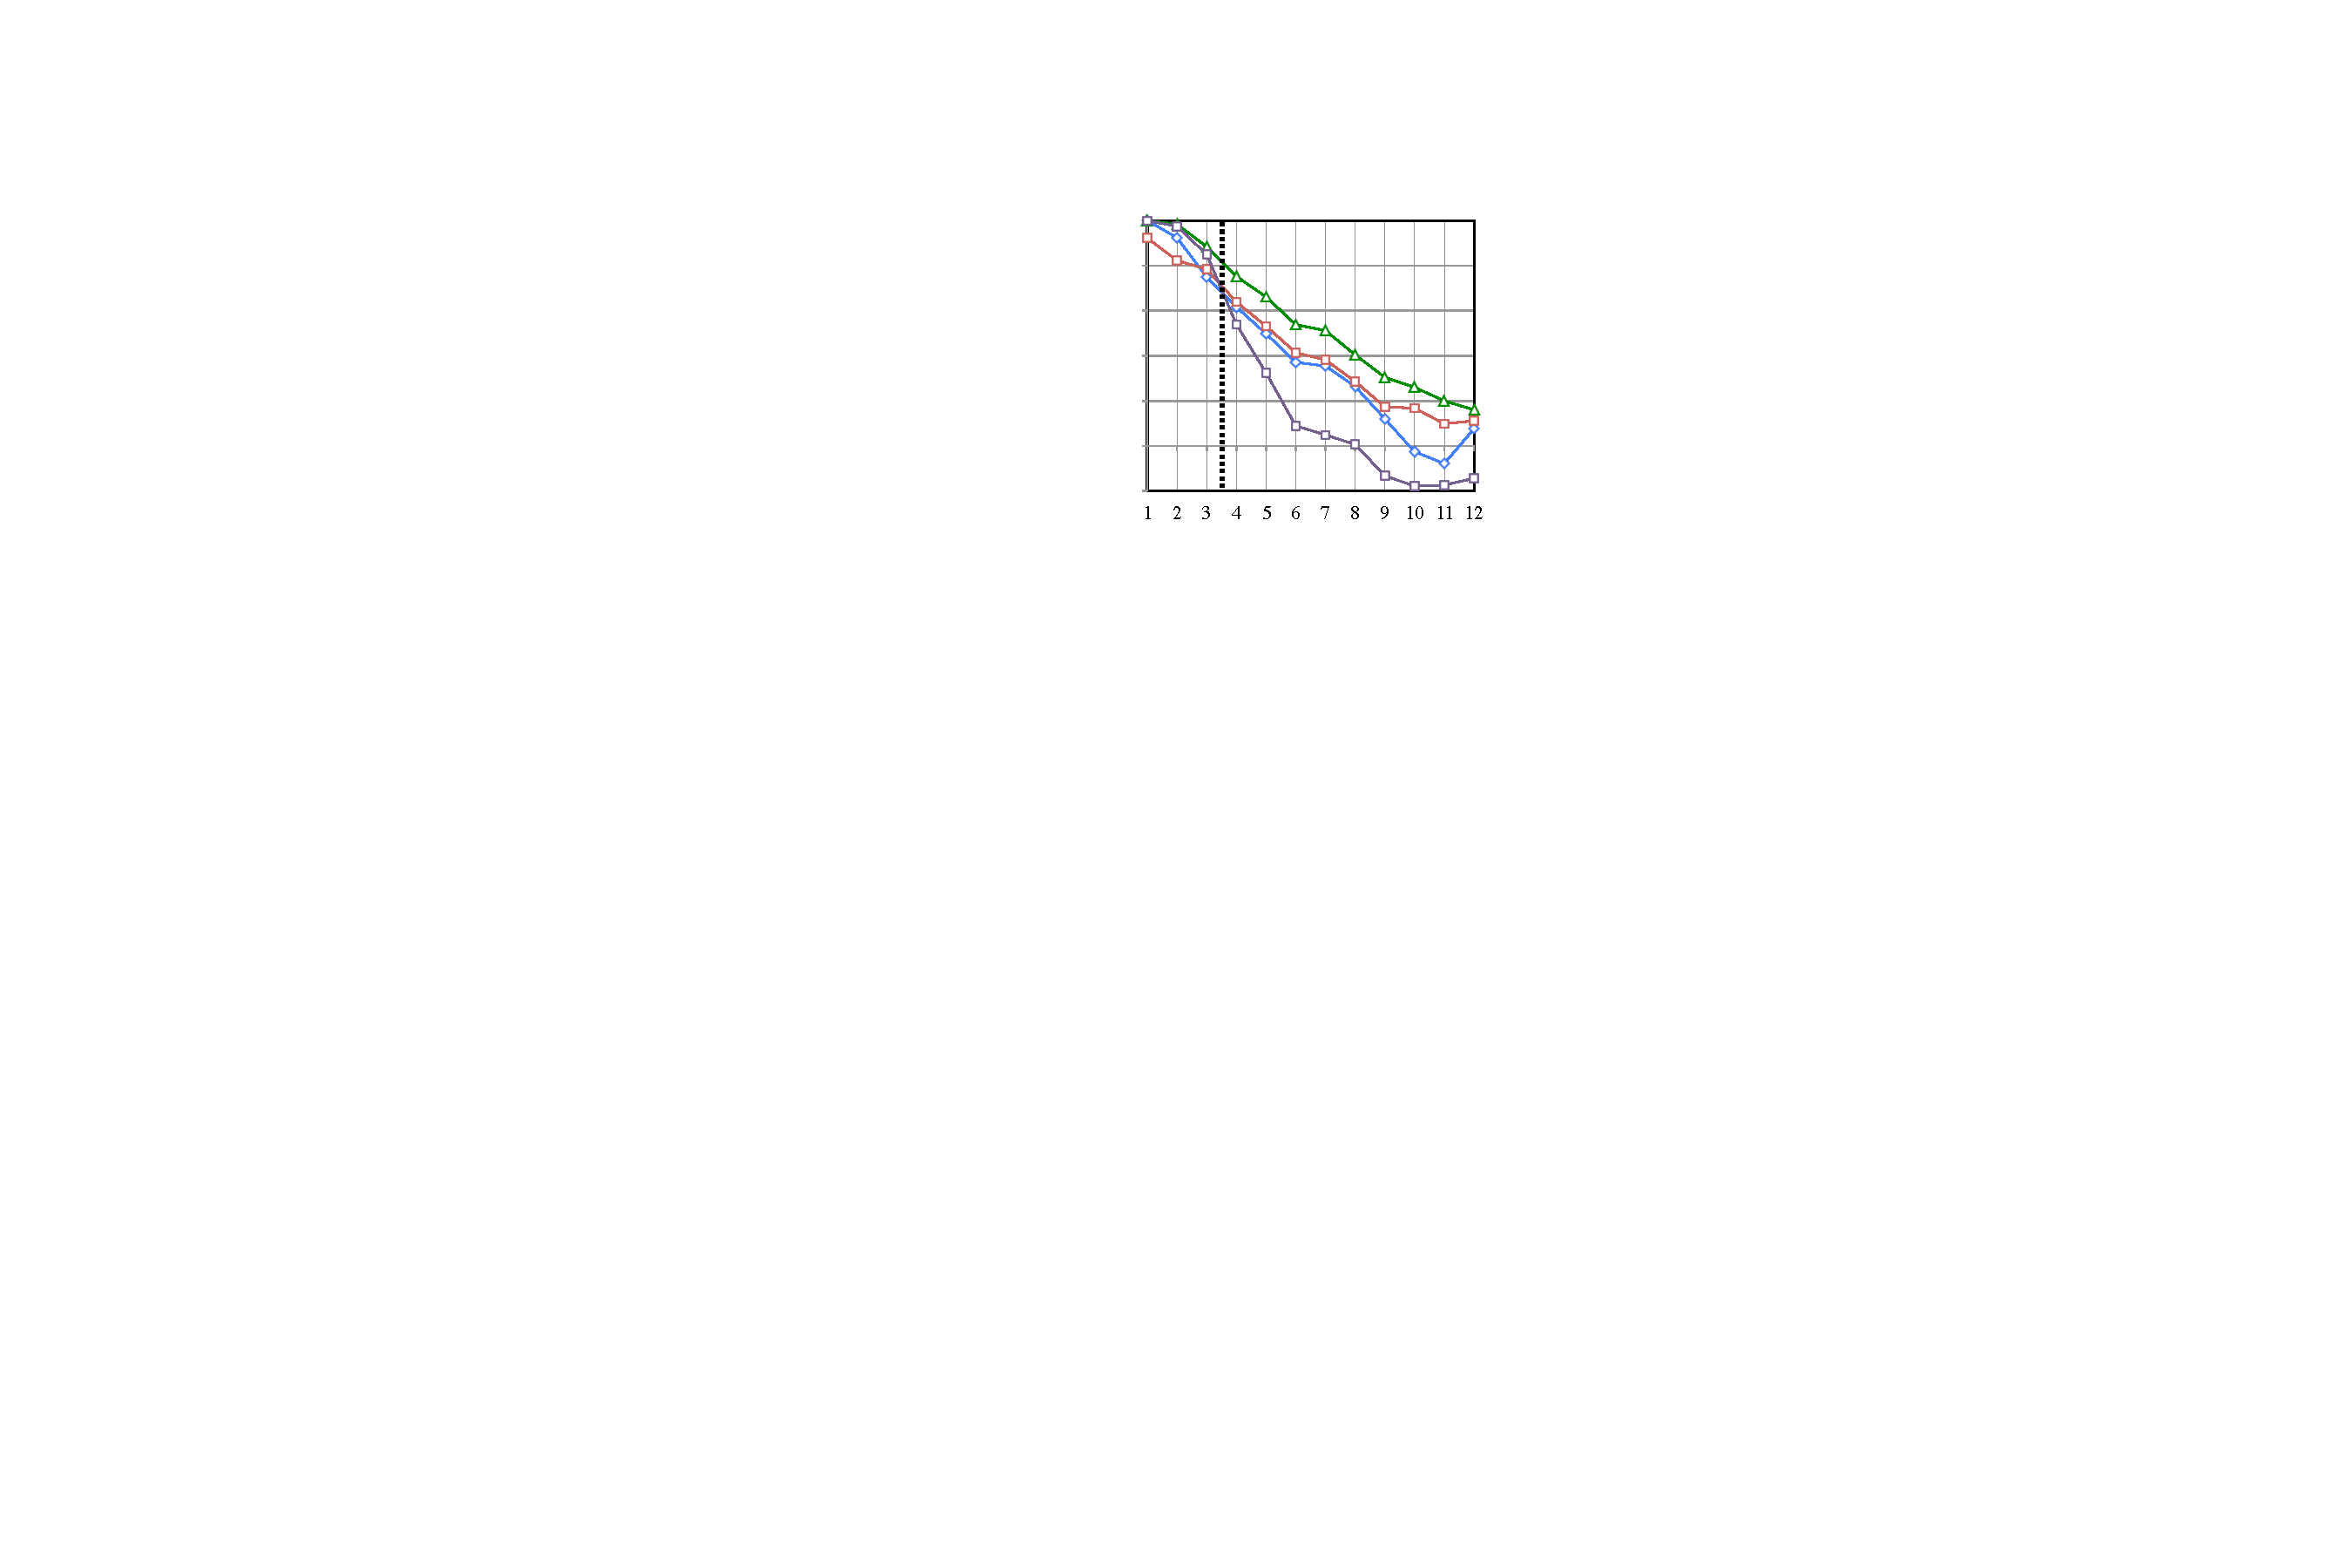
\includegraphics[height=1.6in]{fig3.pdf}
  \caption{Training expression size $\le$3.}
  \end{subfigure}~~
\begin{subfigure}[t]{0.29\textwidth}
    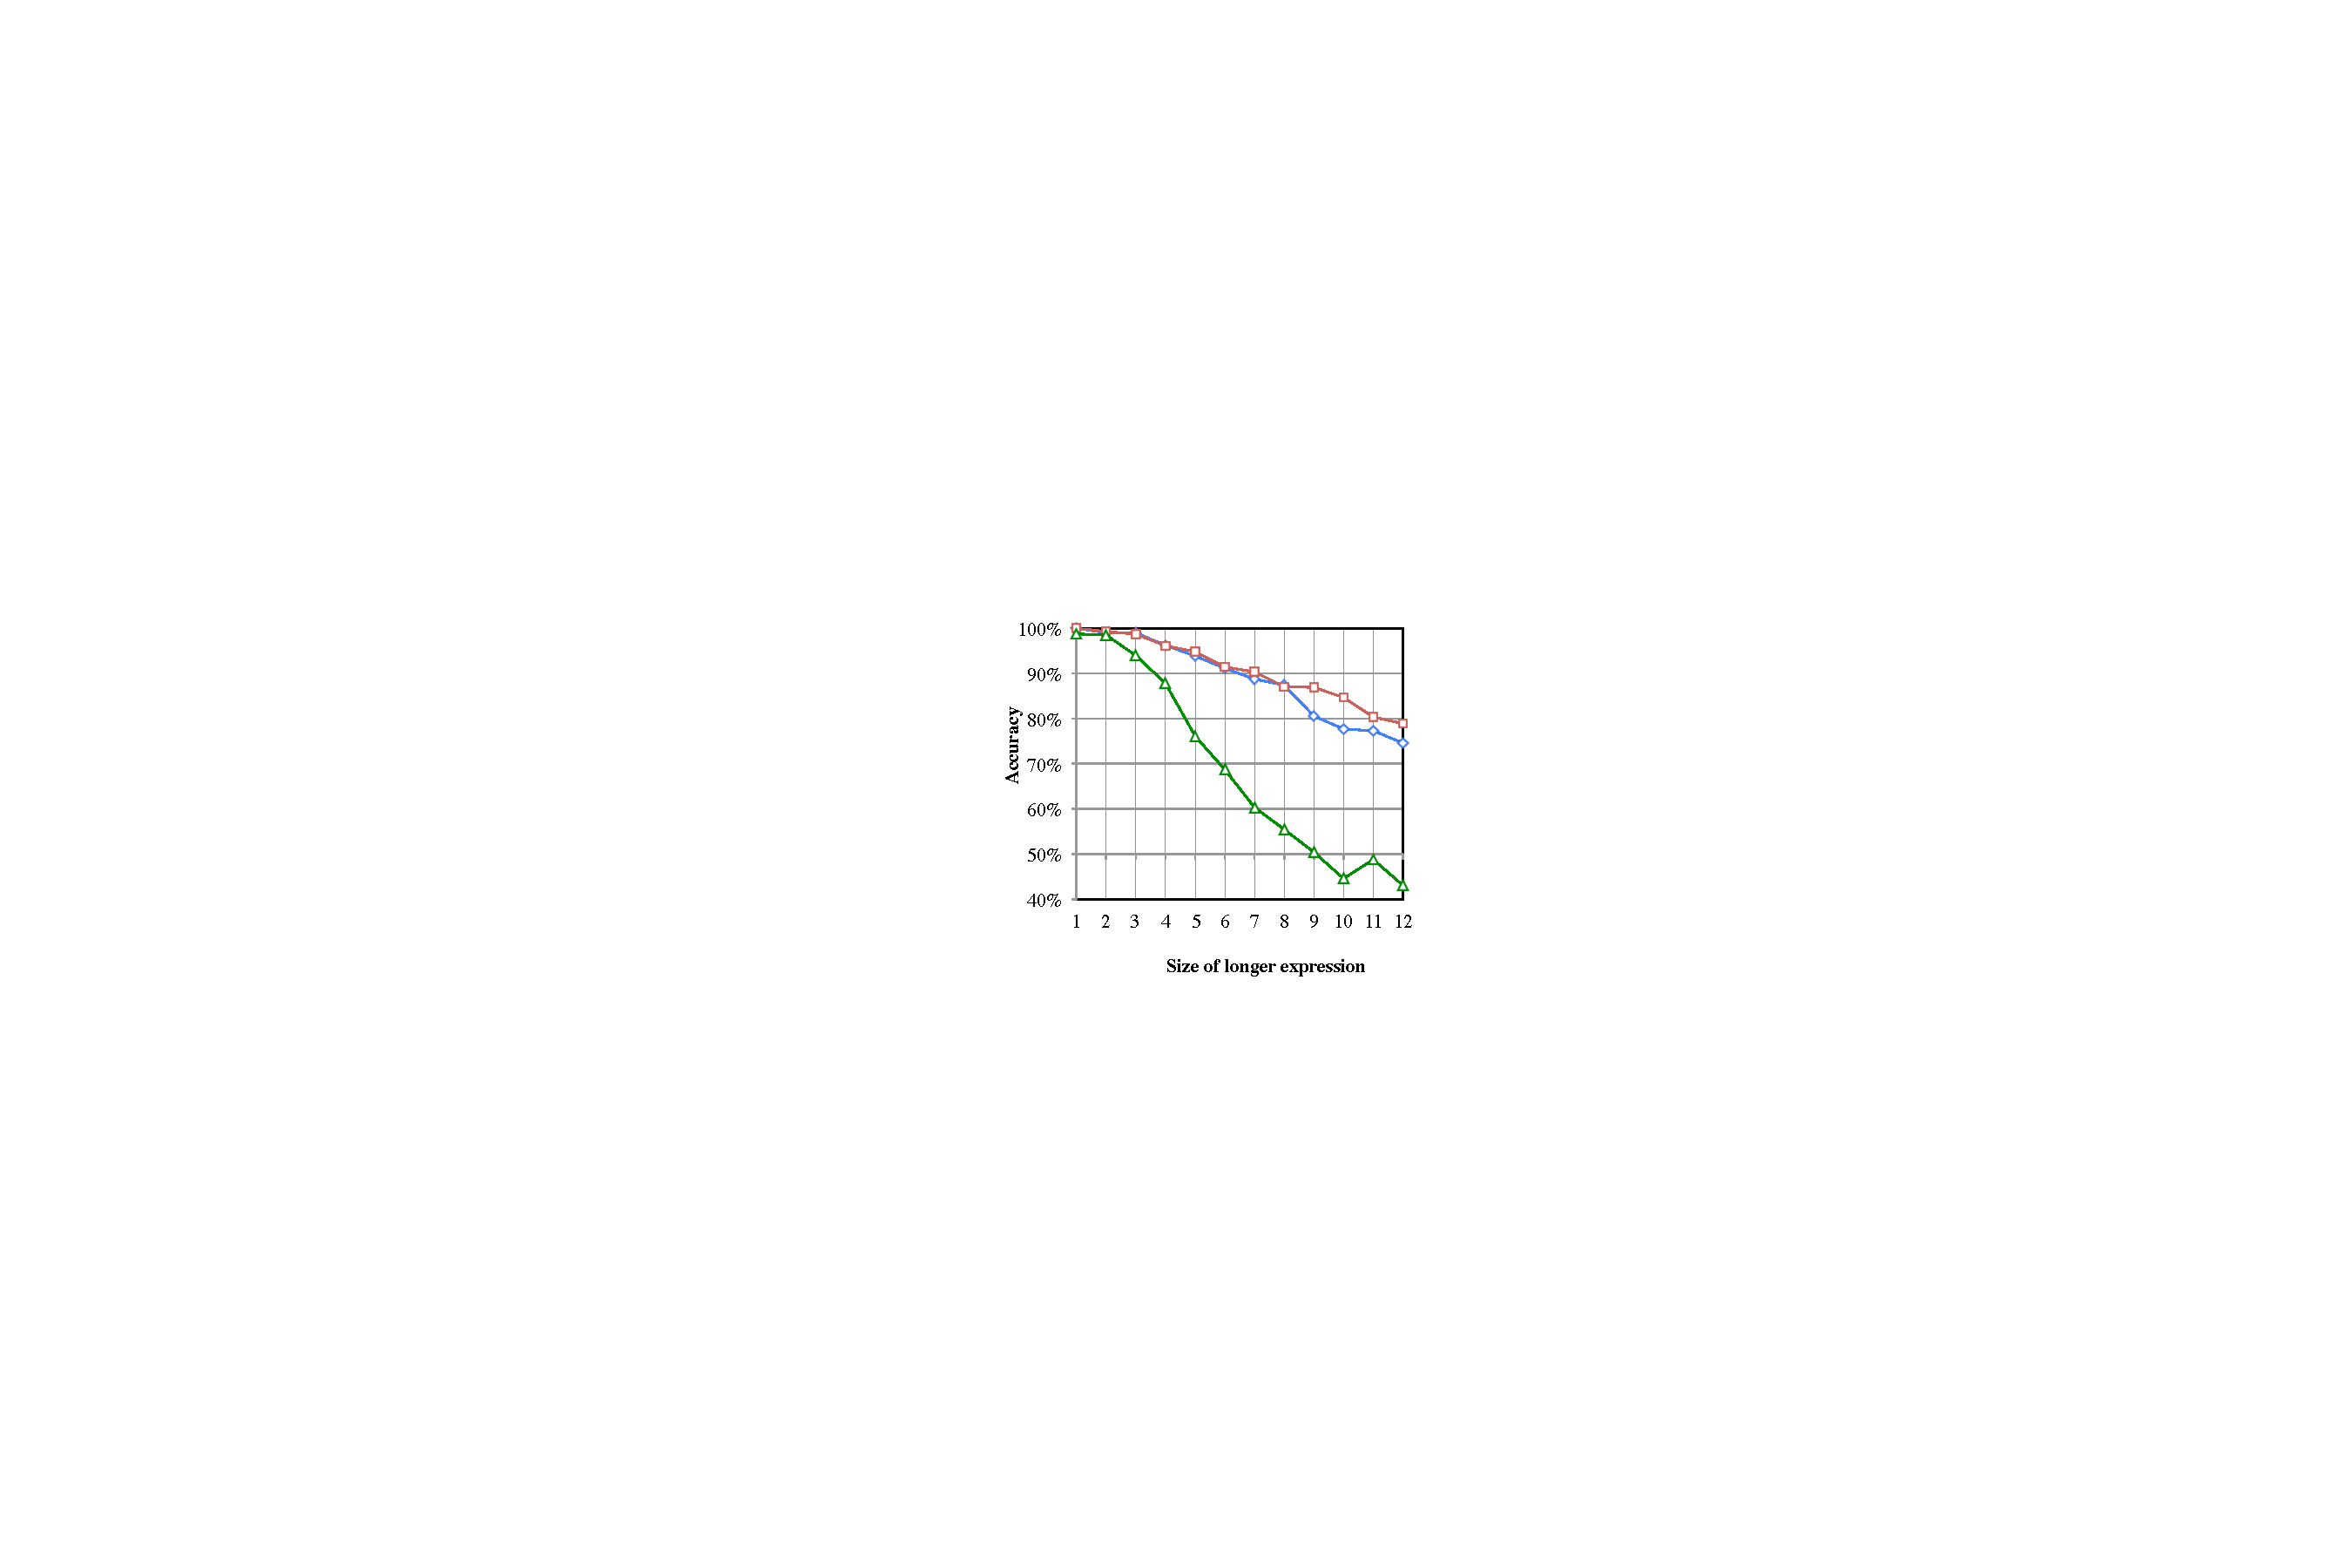
\includegraphics[height=1.6in]{fig4.pdf}
  \caption{Training expression size $\le$4.}
  \end{subfigure}~~
\begin{subfigure}[t]{0.4\textwidth}
      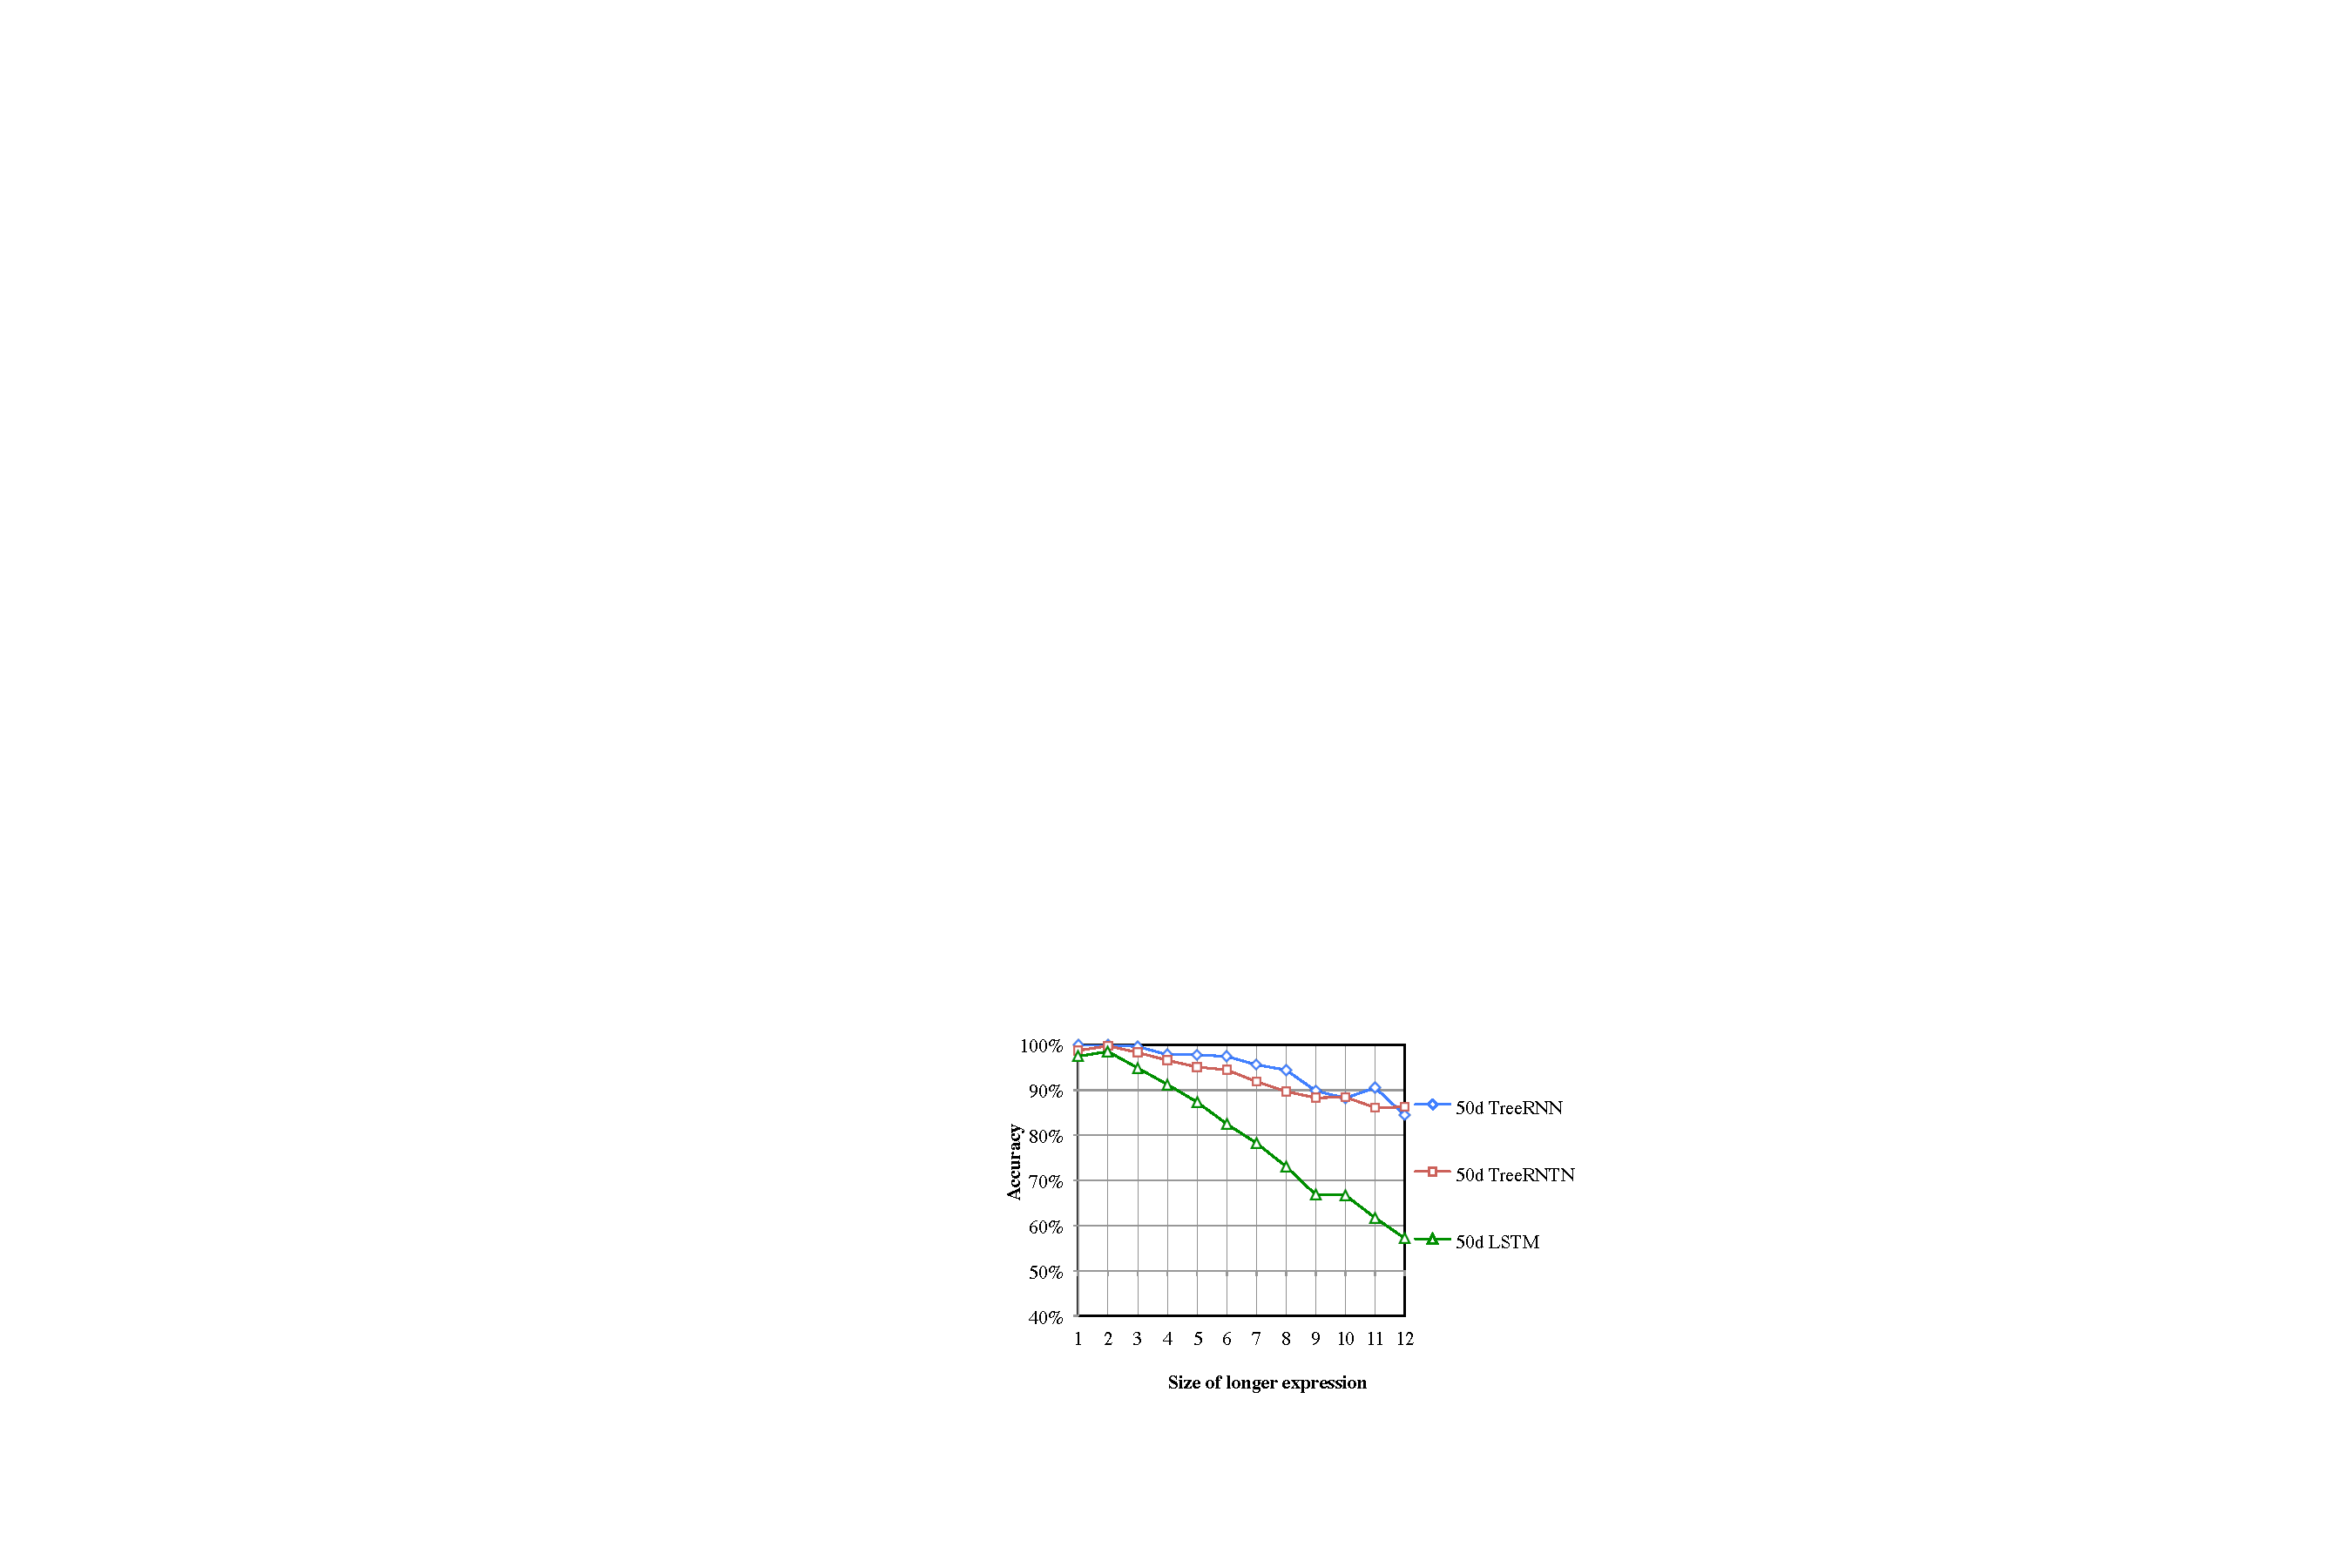
\includegraphics[height=1.6in]{fig6.pdf}
  \caption{Training expression size $\le$6.}
\end{subfigure}
  \caption{Results on three experiments with increasingly rich training sets. The horizontal axis on each graph divides the test set data points (expression pairs) into bins by the number of logical operators in the more complex of the two expressions in the pair.}
  \label{prop-results} 
\end{figure*}

The results are shown in Figure \ref{prop-results}. All three models were able to largely memorize the training data (TODO, TODO, and TODO for $\le$6). With sufficient training data (in the $\le$6 setting), the two tree models were able to perform at above 99\% (TODO) on examples of size $\le$2 with a steady decay in performance continuing through TODO\% at size 12, and similar, if steeper, decays with smaller training sets.

The LSTM performs fairly poorly in the $\le3$ setting, with performance at 3 a mediorce TODO\%, and an abrubt drop to TODO\% at 4, suggesting that the model did not acquire the needed generalizations. With more ample training data in the $\le6$ condition, though, the LSTM shows fairly good accuracy on short examples, and a smooth decay with no abrupt drop. 

\paragraph{Conclusion}

We find that 
